\chapter{质点运动学}
\setcounter{example_counter}{1}

\section{运动学的物理量}

\subsection{位置矢量、轨道}

\subsubsection{位置矢量}

\noindent
\begin{minipage}{0.74\linewidth}
\setlength{\parindent}{2em}
\setlength{\parskip}{0.5em}
\linespread{1.3}
\textbf{位置矢量}:从原点O指向质点位置P的矢量，用$\vec{r}$表示，简称“位矢”。

在直角坐标中，可用三个坐标值$x,y,z$随时间$t$的变化表示质点的运动。

记$\hat{i},\hat{j},\hat{k}$表示$x,y,z$方向的单位向量，则坐标为$(x,y,z)$的质点，位置矢量可表示为

\begin{formula}
    $\vec{r}=x\hat{i}+y\hat{j}+z\hat{k}$
\end{formula}

\end{minipage}
\hfill
\begin{minipage}{0.25\textwidth}
    \vspace{-1em}
    \centering 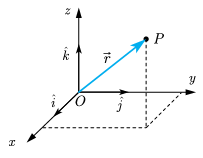
\includegraphics[width=\textwidth]{asset/ch1/T1.png}
\end{minipage}

\subsubsection{轨道}

\textbf{轨道}：质点运动时所经过的路线。只需将$t$消掉，求出$x,y,z$之间的关系。

\begin{example}{求轨道方程}

    根据运动函数求轨道方程：(1)~$\vec{r}=t^2\hat{i}+(2t+3)\hat{j}$ (SI)；(2)~$\vec{r}=\cos^3{t}\hat{i}+\sin^3{t}\hat{j}$ (SI)。
    
    \tcblower

    (1)~根据运动函数，对照$\vec{r}=x\hat{i}+y\hat{j}+z\hat{k}$，可以写出$x=t^2,~y=2t+3$

    \vspace{0.25em}

    根据$y=2t+3$，可以解出$t=\dfrac{(y-3)}{2}$，再代入$x=t^2$，得$x=\dfrac{(y-3)^2}{4}$

    \vspace{0.25em}

    整理得$4x=(y-3)^2$，这就是质点的轨道方程。注：若只考虑$t\geq 0$的运动，则还应有$y\geq 3$.

    (2)~根据运动函数，可写出$x=\cos^3{t},~y=\sin^3{t}$

    利用$\cos^2{t}+\sin^2{t}=1$，可配凑出$x^{\frac{2}{3}}+y^{\frac{2}{3}}=1$，这就是质点的轨道方程。

    \tcbline

    \noindent
    \begin{minipage}{0.78\linewidth}
    \setlength{\parskip}{0.5em}
    \linespread{1.3}
    【补充练习】质点做初速度斜向上$45^\circ$的斜抛运动，坐标系如图所示。根据斜抛运动规律，写出$x,y$随$t$的变化关系，并求质点的轨道方程。
    \end{minipage}
    \hfill
    \begin{minipage}{0.2\textwidth}
        \centering 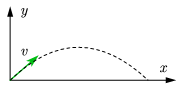
\includegraphics[width=\textwidth]{asset/ch1/T2.png}
    \end{minipage}
    
\end{example}

\subsection{位移与路程}

%\subsubsection{定义}

\noindent
\begin{minipage}{0.83\linewidth}
\setlength{\parskip}{0.5em}
\setlength{\parindent}{2em}
\linespread{1.3}

\textbf{路程}：质点运动的路径长，记为$\Delta s$，路程是标量，只有大小，没有方向。

\textbf{位移}：质点位置的改变量，记为$\Delta \vec{r}$，位移是矢量，既有大小，也有方向。

\warn{在大学物理中，矢量上方的箭头不可省略，位移不能写成$\Delta r$.}
\end{minipage}
\hfill
\begin{minipage}{0.15\textwidth}
    \vspace{-1em}
    \centering 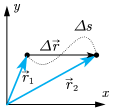
\includegraphics[width=\textwidth]{asset/ch1/T3.png}
\end{minipage}

%\subsubsection{关系}

因为两点之间，直线段最短，所以路程不小于位移的大小。$\Delta s \geq |\Delta \vec{r}|$

但时间$\Delta t \rightarrow 0$时，任意曲线运动可近似为直线运动，$ds = |d \vec{r}|$

\note{当时间足够短，$\Delta t \rightarrow 0$时，$\Delta$符号可改写为$d$符号。}

\warn{若矢量不写箭头，则认为是矢量的大小，$r$表示的是$|\vec{r}|$. 在大学物理阶段，$\Delta |\vec{r}|$、$\Delta r$、$d |\vec{r}|$、$dr$这些写法都是错误的，没有物理意义。位移的大小必须写成$|\Delta \vec{r}|$、$|d \vec{r}|$.}

\subsection{速度与速率}

\subsubsection{速度}

速度是位置的变化率，是单位时间内的位移，是矢量，既有大小，也有方向。

平均速度等于位移除以时间，$\bar{\vec{v}}=\dfrac{\Delta \vec{r}}{\Delta t}$，$\Delta t \rightarrow 0$时的极限，即为瞬时速度$\vec{v}=\dfrac{d\vec{r}}{dt}$

在直角坐标中，可以对三个坐标分别求导，得到速度在三个方向上的分量。

\begin{formula}
    $\vec{v}=\dfrac{d\vec{r}}{dt}=\dfrac{dx}{dt}\hat{i}+\dfrac{dy}{dt}\hat{j}+\dfrac{dz}{dt}\hat{k}$
\end{formula}

\subsubsection{速率}

速率是单位时间内的路程，是标量，只有大小，没有方向。

平均速率等于路程除以时间，$\bar{v}=\dfrac{\Delta s}{\Delta t}$，$\Delta t \rightarrow 0$时的极限称为瞬时速率$v=\dfrac{ds}{dt}$

\subsubsection{速度与速率的关系}

因为$\Delta s \geq |\Delta \vec{r}|$，所以平均速率不小于平均速度的大小。

但是$ds = |d \vec{r}|$，所以瞬时速率等于瞬时速度的大小。

\begin{example}{速度与速率的定义}
    质点在$xy$平面上运动。下列写法中，哪些表示瞬时速度，哪些表示瞬时速率？

    \vspace{0.3em}

    A. $\dfrac{d \vec{r}}{dt}$~~~B. $\dfrac{d |\vec{r}|}{dt}$~~~C. $\dfrac{dr}{dt}$~~~D. $\left|\dfrac{d\vec{r}}{dt}\right|$~~~E. $\dfrac{ds}{dt}$~~~F. $\dfrac{dx}{dt}+\dfrac{dy}{dt}$~~~G. $\sqrt{\left(\dfrac{dx}{dt}\right)^2+\left(\dfrac{dy}{dt}\right)^2}$

    \tcblower

    A是瞬时速度的定义，E是瞬时速率的定义，D是瞬时速度的大小，表示瞬时速率。
    
    B和C出现了$d |\vec{r}|$、$dr$的错误写法，无物理意义。

    \vspace{0.3em}

    $\dfrac{dx}{dt}$、$\dfrac{dy}{dt}$分别表示速度在$x,y$方向的分量$v_x,v_y$，合成时应采用勾股定理，而非直接相加。

    \vspace{0.3em}
    
    因此G选项表示瞬时速率，F选项无物理意义。

    \tcbline

    【补充练习】质点做半径为$R$的匀速圆周运动，周期为$T$，求$t=2T$时间内的位移、路程、平均速度、平均速率。
    
\end{example}

\subsection{加速度}

加速度是速度的变化率，也可分为平均加速度和瞬时加速度。

平均加速度等于速度的变化量除以时间，$\overline{\vec{a}}=\dfrac{\Delta \vec{v}}{\Delta t}$，$\Delta t \rightarrow 0$时的极限称为瞬时加速度$\vec{a}=\dfrac{d\vec{v}}{dt}$

在直角坐标系中，分别对$x,y,z$求二阶导（即两次求导），得到的就是加速度在三个方向上的分量。

\begin{formula}
    $\vec{a}=\dfrac{d\vec{v}}{dt}=\dfrac{d^2\vec{r}}{dt^2}=\dfrac{d^2x}{dt^2}\hat{i}+\dfrac{d^2y}{dt^2}\hat{j}+\dfrac{d^2z}{dt^2}\hat{k}$
\end{formula}


\begin{itemize}
    \item 对于直线运动而言，速度与加速度同向时加速，反向时减速。不是加速度为正时加速，为负时减速。
    \item 对于曲线运动，速度与加速度夹角小于$90^\circ$时加速，大于$90^\circ$时减速。
\end{itemize}

\subsection{运动学的两类基本问题}

位置矢量$\vec{r}$、速度$\vec{v}$、加速度$\vec{a}$的关系如下。知道一个物理量随时间的关系，即可求出另外两个。

\note{如无特殊说明，速度、加速度默认都是指瞬时速度、加速度。}

\begin{figure}[htb]
    \centering
    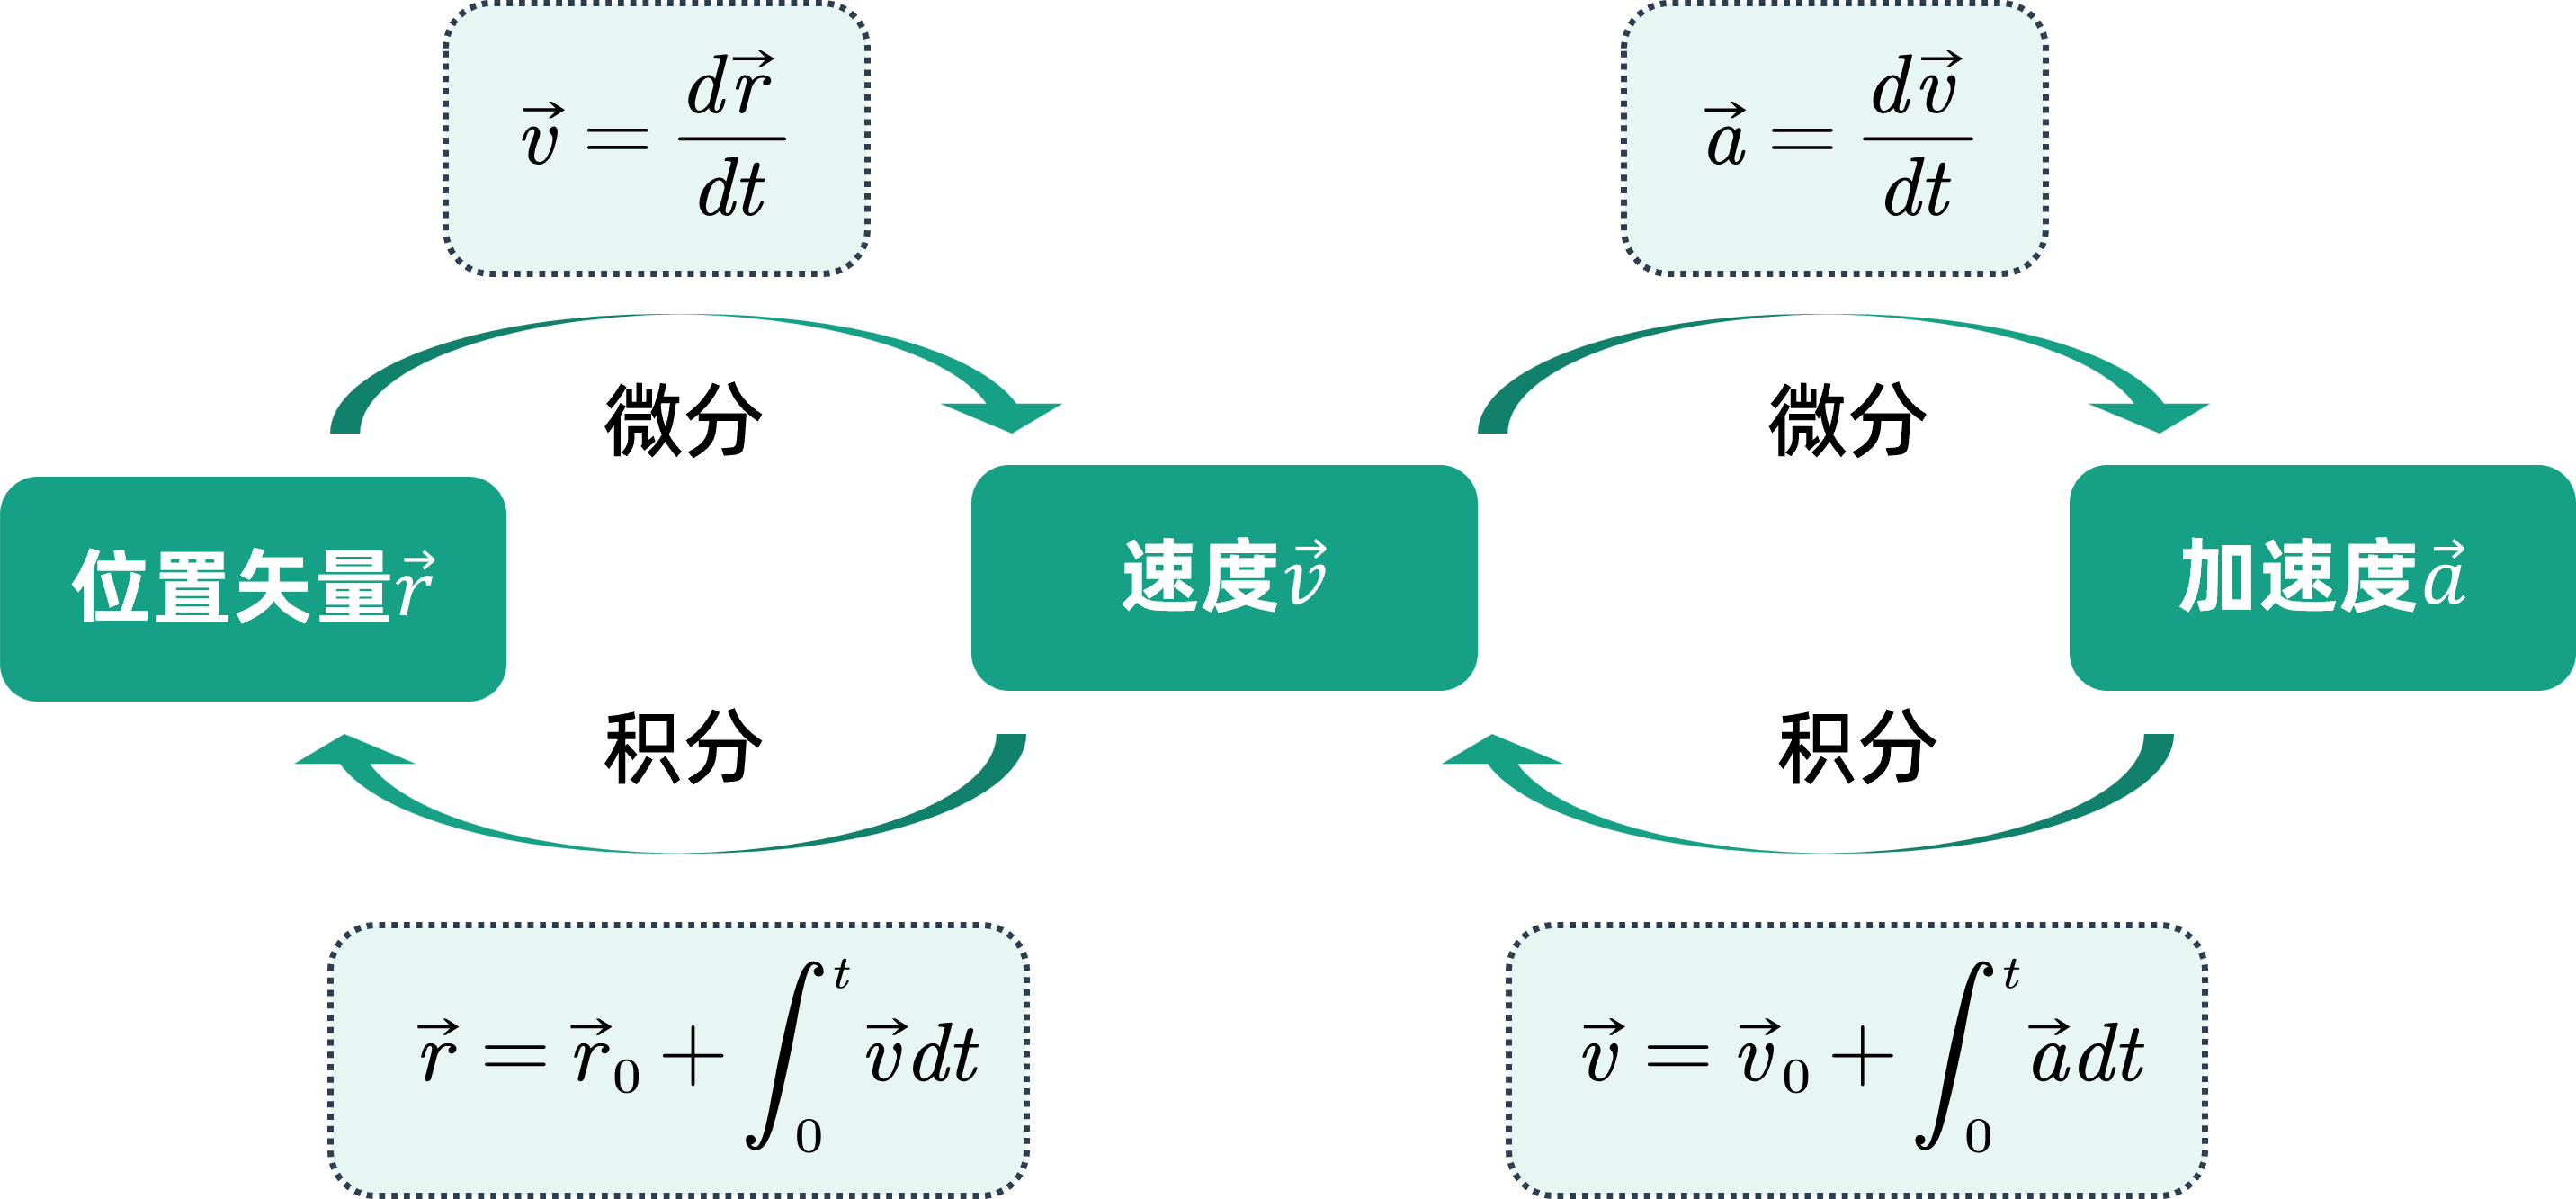
\includegraphics[width=0.65\linewidth]{asset/ch1/T4.png}
\end{figure}

\warn{注意在积分求解时，不要忘了考虑初始条件。}

\begin{example}{运动学第一类问题}
    运动函数为$\vec{r}=(3t+5)\hat{i}+(t^2+3t−4)\hat{j}$(SI)，求：$t=\SI{4}{s}$时的速度和加速度，前$\SI{4}{s}$的平均速度。

    \tcblower

    根据质点运动函数，可写出$x=3t+5,~y=t^2+3t−4$

    \vspace{0.25em}
    
    求导可得$v_x=\dfrac{dx}{dt}=3,~v_y=\dfrac{dy}{dt}=2t+3$，再次求导可得$a_x=\dfrac{d^2x}{dt^2}=0,~a_y=\dfrac{d^2y}{dt^2}=2$

    \vspace{0.3em}

    将$t=\SI{4}{s}$，代入，可得$v_x=3,~v_y=11,a_x=0,~a_y=2$，可写成$\vec{v}=3\hat{i}+11\hat{j},~\vec{a}=2\hat{j}$

    要求平均速度，需要先求位移。当$t=0,\SI{4}{s}$时，$\vec{r}_1=5\hat{i}-4\hat{j},~\vec{r}_2=17\hat{i}+24\hat{j}$

    \vspace{0.3em}

    所以位移$\Delta \vec{r}=\vec{r}_2-\vec{r}_1=12\hat{i}+28\hat{j}$，平均速度$\bar{\vec{v}}=\dfrac{\Delta \vec{r}}{\Delta t}=3\hat{i}+7\hat{j}$
    
    \tcbline
    【补充练习】已知质点运动方程为$x=2t,~y=2-t^2$，求：(1)~前$\SI{2}{s}$内的平均速度、第$\SI{2}{s}$末的速度；(2)~前$\SI{2}{s}$内的平均加速度、第$\SI{2}{s}$末的加速度。
\end{example}

\begin{example}{运动学第二类问题}
    质点沿$x$轴运动，加速度$a=-6t$~(SI)。已知$t=\SI{3}{s}$时，$x=\SI{-12}{m},~v=\SI{-24}{m/s}$，求： (1)~求任意时刻的速度和位置；(2)~判断什么时候向正方向运动，什么时候向负方向运动（只考虑$t\geq 0$）；(3)~判断什么时候加速、什么时候减速；(4)~求前$\SI{2}{s}$内的路程、位移、平均速度、平均速率。

    \tcblower

    (1)~~将$a$对$t$求积分，可得$v=v_0+\displaystyle \int_0^t{(-6t)dt}=v_0-3t^2$

    \vspace{0.25em}
    
    代入$t=3$时$v=-24$，得$v_0=3$，因此$v=3-3t^2$

    \vspace{0.25em}

    再将$v$对$t$求积分，可得$x=x_0+\displaystyle \int_0^t{(3-3t^2)dt}=x_0+3t-t^3$

    \vspace{0.25em}
    
    代入$t=3$时$x=-12$，得$x_0=6$，因此$x=3t-t^3+6$
    \note{在一维问题中，矢量运算退化成标量运算，可省略上方的箭头，用正负表示其方向。}

    (2)~~当$v>0$时，即$0\leq t<\SI{1}{s}$时，向正方向运动；而$v<0$时，即$t>\SI{1}{s}$时，向负方向运动。

    (3)~~因为$a=-6t<0$，因此当$0\leq t<\SI{1}{s}$时，$v>0$，加速度与速度反向，为减速；
    
    而$t>\SI{1}{s}$时，$v<0$，加速度与速度同向，为加速。

    (4)~~当$t=0,\SI{1}{s},\SI{2}{s}$时，代入表达式可求出$x=\SI{6}{m},\SI{8}{m},\SI{4}{m}$

    位移就是位置变化量，只看初末状态即可，$\Delta x=\SI{4}{m}-\SI{6}{m}=\SI{-2}{m}$

    路程需要按转向时刻分段求解，第$\SI{1}{s}$路程为$\SI{2}{m}$，第$\SI{2}{s}$路程为$\SI{4}{m}$，因此总路程为$\SI{6}{m}$

    平均速度等于位移除以时间，等于$\SI{-1}{m/s}$；平均速率等于路程除以时间，等于$\SI{3}{m/s}$.

    \tcbline
    【补充练习】质点从$\vec{r}=−5\hat{j}$处出发，初速度$\vec{v}=2\hat{i}$。加速度与时间的关系为$\vec{a}=t^2\hat{i}+(2t+3)\hat{j}$(SI)，求：质点在$t=\SI{2}{s}$时的速度和位置矢量。
\end{example}

\section{圆周运动}

\subsection{圆周运动的描述}

在圆周运动中，我们更关心转过角度的变化，因此可以将位置、速度、加速度推广为角位置$\theta$、角速度$\omega$、角加速度$\alpha$，它们之间的微分、积分关系完全相同。

\begin{figure}[htb]
    \centering
    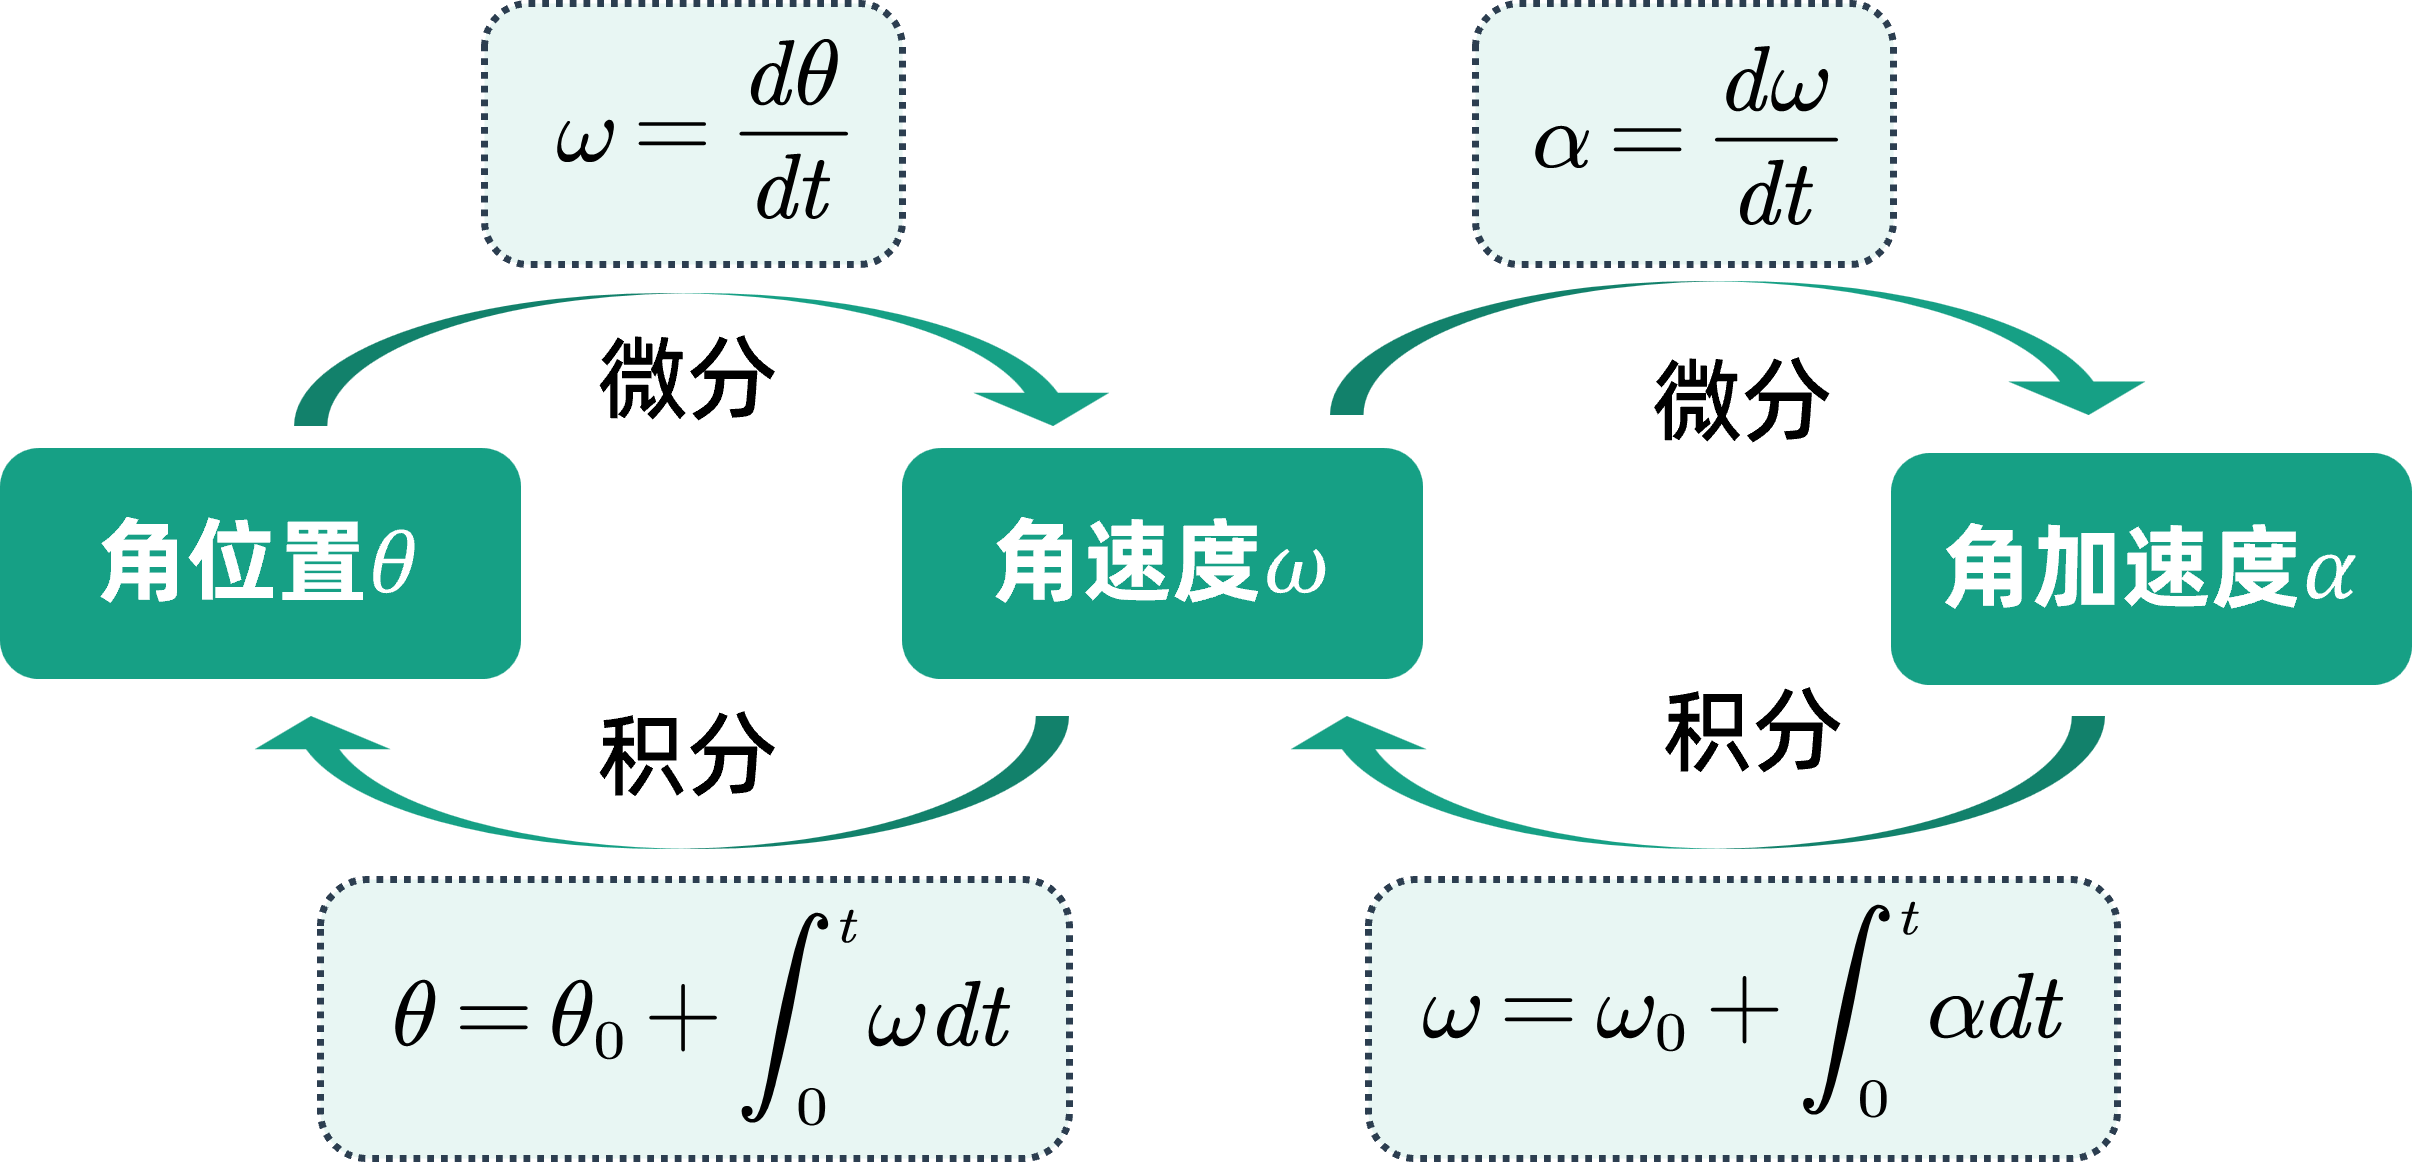
\includegraphics[width=0.65\linewidth]{asset/ch1/T8.png}
\end{figure}

\note{一些教材将角加速度记为符号$\beta$，但国家标准规定为$\alpha$.}

\note{角速度$\omega$是矢量，方向用右手螺旋判断，但大学物理不强调其矢量性。}

%\begin{formula}
%    $\omega=\dfrac{d\theta}{dt},~\alpha=\dfrac{d\omega}{dt},~\theta=\theta_0+\displaystyle\int_0^t{\omega dt},~\omega=\omega_0+\displaystyle\int_0^t{\alpha dt}$
%\end{formula}

\subsection{线量与角量的关系}

路程$s$与角位移$\theta$、线速度$v$与角速度$\omega$的换算只需乘除一个半径$R$，速度的方向为切线方向。

\begin{formula}
    $s=\theta R,~v=\dfrac{ds}{dt}=\omega R$
\end{formula}

但加速度$a$需要分解为切向和法向分别计算：

\begin{itemize}
    \item 切向加速度$a_t$：控制速度大小的变化，是速率的变化率，与速度同向时加速，反向时减速
    \item 法向加速度$a_n$：控制速度方向的变化，指向圆心，即向心加速度
\end{itemize}

%切向与法向加速度的定量表达式为：

\begin{formula}
    $a_t=\dfrac{dv}{dt}=\alpha R,~a_n=\dfrac{v^2}{R},~a=\sqrt{a_t^2+a_n^2}$
\end{formula}

\warn{注意求加速度时，一定要分别求出两个分量，再做合成，而不能直接用角加速度乘以半径。}

\begin{example}{圆周运动}
    质点做$R=2$的圆周运动，静止出发，角加速度与时间的关系为$\alpha=12t^2−6t$（SI）
    
    (1) 求任意时刻的角速度、角位移；(2) 求$t=2$时刻的线速度和加速度的大小。
    \tcblower
    
    (1)~静止出发可知初始$\omega_0=0$，对角加速度积分可得角速度，$\omega=0+\displaystyle\int_0^t{(12t^2-6t)dt}=4t^3-3t^2$

    %\vspace{0.25em}

    再求一次积分，即可得到角位移
    $\theta=0+\displaystyle\int_0^t{(4t^3-3t^2)dt}=t^4-t^3$

    \vspace{0.25em}

    (2)~代入$t=2$，可得$\alpha=36,~\omega=20$，根据线量与角量的关系，$v=\omega R=40$

    \vspace{0.25em}

    加速度需要分别求切向和法向，$a_t=\alpha R=72,~a_n=\dfrac{v^2}{R}=800$，合成可得$a=\sqrt{a_t^2+a_n^2}\approx 803$
    \tcbline
    【补充练习】质点做$R=3$的圆周运动，路程与时间的关系为$s=3t+3t^2$，始终逆时针运动。(1)~求$t=2$时刻的线速度、角速度、加速度、角加速度的大小；(2)~在哪一时刻，加速度与速度方向的夹角为$45^\circ$？
\end{example}

\section{相对运动}

仅考虑参考系相对于大地平动的情况，变换参考系前后，可定义三种速度：
\begin{itemize}
    \item \textbf{绝对速度}：质点相对于大地的速度
    \item \textbf{相对速度}：质点相对于选定参考系的速度
    \item \textbf{牵连速度}：选定参考系相对于大地的速度
\end{itemize}

这三种速度之间的关系是

\begin{formula}  
   $\text{绝对}=\text{相对}+\text{牵连}$
\end{formula}


\note{上式的加法应理解为矢量相加，位移、加速度也满足类似的关系。}

\begin{example}{相对运动}
    某人以速度$v$向西匀速骑车，有风从北偏东$30^\circ$方向以相同速率吹来，这个人感受到的风来自什么方向，风速如何？
    \tcblower

    空气流动产生了风，以空气为研究对象，风的速度是空气相对于大地的速度，是绝对速度。

    \vspace{0.7em}

    \noindent
    \begin{minipage}{0.78\linewidth}
    \setlength{\parskip}{0.5em}
    \linespread{1.1}
    
    而人感受到的风，应是空气相对于人的速度，是相对速度。

    此时，参考系应变换到人的身上，因此人相对于大地的速度是牵连速度。

    根据题意，结合绝对=相对+牵连的关系，可画出三者之间的关系如右图所示。因此人感受到的风，即相对速度，为北偏西$30^\circ$方向，大小为$v$.
    \end{minipage}
    \hfill
    \begin{minipage}{0.2\textwidth}
        \centering 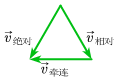
\includegraphics[width=\textwidth]{asset/ch1/T10.png}
    \end{minipage}
    
    \tcbline
    【补充练习】以正东、正北为$x,y$轴正方向。甲乙两船以$\SI{2}{m/s}$的速率匀速行驶，甲向正东方向运动，乙向北偏东$30^\circ$方向运动。求乙相对于甲的速度。
\end{example}

\section{拓展内容}

\subsection{运动学的实际问题}

在一个实际场景中，要求某点的速度或加速度，可建立坐标系，利用该点的坐标建立几何关系，再对等号两边同时求导，即可得到未知点与已知点之间的速度、加速度关系。

\note{注意$x,y$是时间的函数，求导时要用隐函数求导法则。例如$x^2$求导的结果不是$2x$，而是$2x\dfrac{dx}{dt}$.}

\begin{example}{运动学实际问题*}
    一人通过岸边的定滑轮（大小可忽略）用绳子拉船，使船靠岸，假定绳子不可伸长且始终绷紧，拉绳的速率恒为$u$，水面与滑轮的高度差为$H$.~求当绳与水平面夹角为$\theta$时，船运动的速度和加速度。
    \tcblower
    
    \noindent
    \begin{minipage}{0.73\linewidth}
    \setlength{\parskip}{0.5em}
    \linespread{1.3}
    建立如图所示的坐标系，设船的横坐标为$x$，滑轮到船之间的绳长为$L$
    
    则根据勾股定理，$x^2+H^2=L^2$，根据题意，绳缩短的速率$\dfrac{dL}{dt}=-u$

    {\fangsong 注：$\dfrac{dL}{dt}=-u$并不表示某一质点的速度，而是绳长对时间的变化率}

    \vspace{-0.1em}

    \end{minipage}
    \hfill
    \begin{minipage}{0.25\textwidth}
        \centering 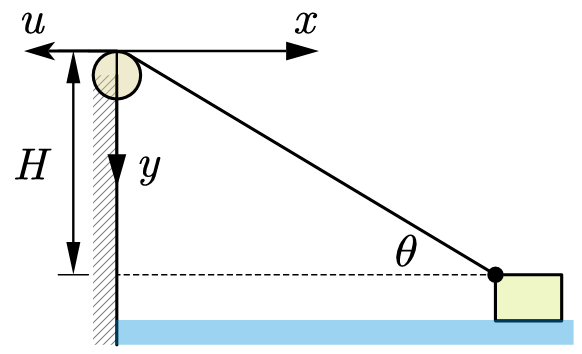
\includegraphics[width=\textwidth]{asset/ch1/T12.png}
    \end{minipage}

    对两边分别求导得$2x\dfrac{dx}{dt}+0=2L\dfrac{dL}{dt}$，解得$v=\dfrac{dx}{dt}=-\dfrac{L}{x}u=-\dfrac{u}{\cos{\theta}}$

    对$x\dfrac{dx}{dt}=L\dfrac{dL}{dt}$两边再求导，得$\left(\dfrac{dx}{dt}\right)^2+x\dfrac{d^2x}{dt^2}=\left(\dfrac{dL}{dt}\right)^2+L\dfrac{d^2L}{dt^2}$

    \vspace{0.3em}

    而其中$\dfrac{d^2L}{dt^2}=0$，代入整理得$a=\dfrac{d^2x}{dt^2}=\dfrac{u^2-v^2}{x}=\dfrac{u^2(1-1/\cos^2\theta)}{H/\tan\theta}=-\dfrac{u^2\tan^3{\theta}}{H}$
    
    \tcbline
    
    \noindent
    \begin{minipage}{0.78\linewidth}
    \setlength{\parskip}{0.5em}
    \linespread{1.3}
    【补充练习】长为$L$的木棍靠在墙上，慢慢滑落。记木棍下端为A点、上端为B点，假设A点的移动速度恒为$v$。某一时刻，木棍与水平方向夹角为$\theta$。求B点此时的速度和加速度。
    \end{minipage}
    \hfill
    \begin{minipage}{0.2\textwidth}
        \centering 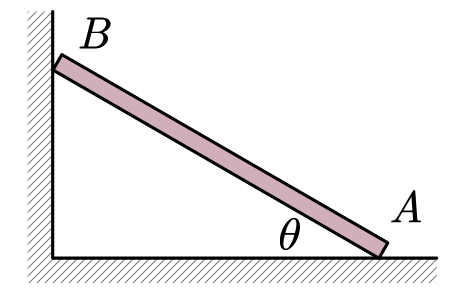
\includegraphics[width=\textwidth]{asset/ch1/T6.png}
    \end{minipage}
\end{example}

\subsection{曲线运动与自然坐标系}

\noindent
    \begin{minipage}{0.73\linewidth}
    
    \setlength{\parskip}{0.5em}
    \setlength{\parindent}{2em}
    \linespread{1.3}
    \subsubsection{自然坐标系}

    \vspace{1em}
    
    若质点做曲线运动，可沿轨道建立坐标系，选定原点O后，用曲线长度$s$表示质点的位置，这种坐标系称为\textbf{自然坐标系}。
    \end{minipage}
    \hfill
    \begin{minipage}{0.25\textwidth}
        \centering 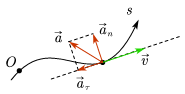
\includegraphics[width=\textwidth]{asset/ch1/T7.png}
    \end{minipage}

在任意时刻，速度方向为曲线的切线方向，大小（即速率）等于$v=\dfrac{ds}{dt}$

\subsubsection{曲线运动的加速度}

在曲线运动中，曲线上各点都可以找到一个贴合最好的圆，称为“曲率圆”，其半径称为“曲率半径”，用$\rho$表示。因此，曲线运动的每一小段都可近似为一个圆周运动，从而求出切向和法向加速度。

\begin{itemize}
    \item 切向加速度：控制速度大小的变化，是速率的变化率，$a_t=\dfrac{dv}{dt}$
    \item 法向加速度：控制速度方向的变化，指向曲线凹侧，$a_n=\dfrac{v^2}{\rho}$
\end{itemize}

\warn{注意加速度是速度的变化率，而切向加速度是速率的变化率。}

在自然坐标系下，曲线运动的速度和加速度的定量表达式总结如下。

\begin{formula}
    $v=\dfrac{ds}{dt},~a_t=\dfrac{dv}{dt},~a_n=\dfrac{v}{\rho^2}$
\end{formula}

\begin{example}{自然坐标系*}
    质点以$\SI{10}{m/s}$的速度水平抛出，做平抛运动。当速度方向与水平方向成$60^\circ$角时，求瞬时速率、速度变化率、速率的变化率、曲率半径。（取$g=\SI{10}{m/s^2}$）
    \tcblower
    
    \begin{minipage}{0.78\linewidth}
    
    \setlength{\parskip}{0.5em}
    
    \linespread{1.3}
    根据平抛运动的规律，水平方向做匀速直线运动，因此$v=\dfrac{v_x}{\cos{60^\circ}}=\SI{20}{m/s}$

    \vspace{0.25em}

    速度的变化率就是瞬时加速度，而平抛运动的加速度是重力加速度，大小为$a=g=\SI{10}{m/s^2}$，方向竖直向下，这就是速度的变化率。

    加速度可在平行和垂直速度的方向上进行分解。
    
    切向加速度$a_t=a\sin{30^\circ}=5\sqrt{3}\unit{m/s^2}$，这就是速率的变化率。

    \vspace{0.3em}

    法向加速度$a_n=a\cos{30^\circ}=\SI{5}{m/s^2}$，利用$a_n=\dfrac{v^2}{\rho}$，得曲率半径$\rho=\SI{80}{m}$

    \end{minipage}
    \hfill
    \begin{minipage}{0.2\textwidth}
        \centering 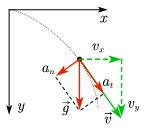
\includegraphics[width=\textwidth]{asset/ch1/T11.png}
    \end{minipage}
    
    \tcbline
    【补充练习】质点运动方程为$x=3t, y=12−3t^2$(SI)，求$t=\SI{1}{s}$时的瞬时速度、速度的变化率、速率的变化率和曲率半径。
\end{example}